\chapter{Galerie}



\begin{figure}[ht]
    \centering
    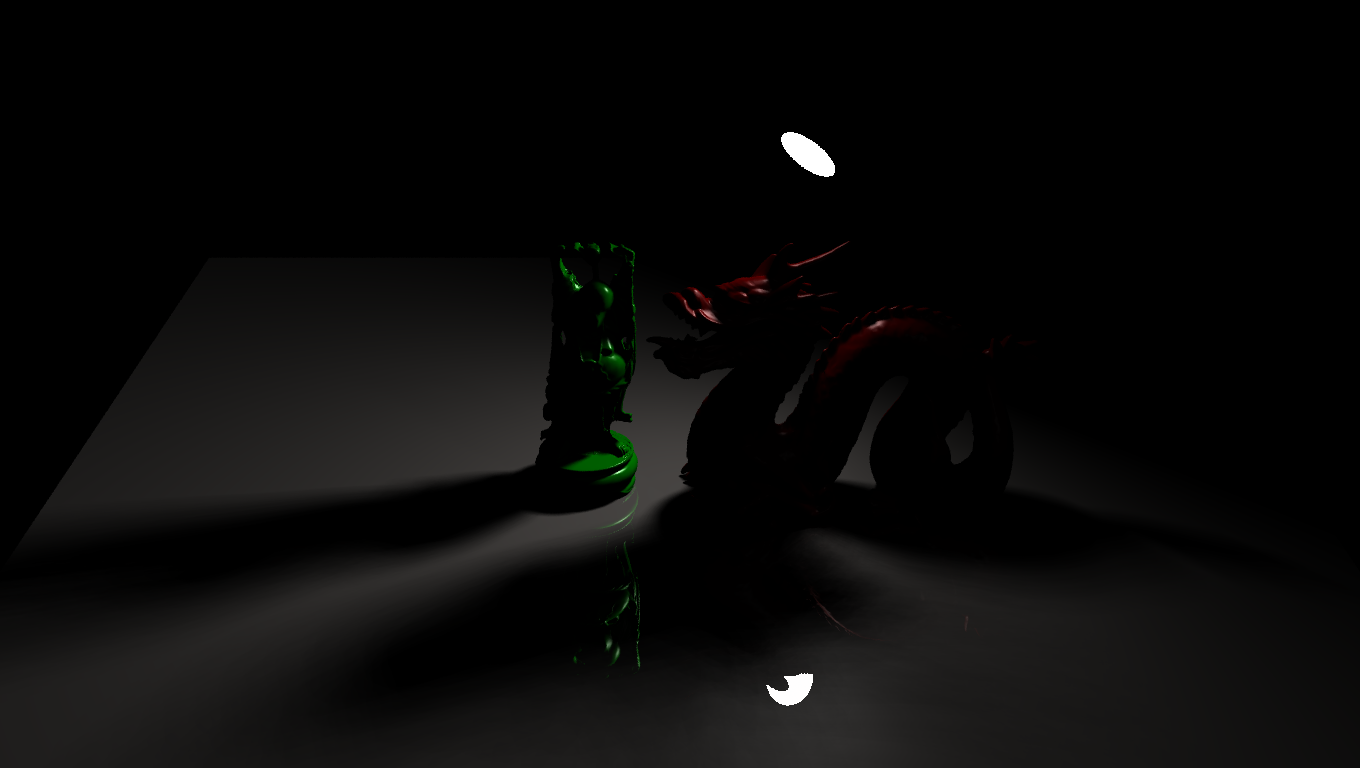
\includegraphics[width=1\textwidth]{./img/galerie/bhudda_dragon_glossy_plane_dark}
    \caption{Phong schattierter "`Stanford Buddha"' und "`Stanford Dragon"' auf spiegelndem Untergrund. Die Szene wird von zwei runden Flächenlichter beleuchtet.}
    \label{fig:bhudda_dragon_plane_glossy_dark}
\end{figure}



\begin{figure}[ht]
    \centering
    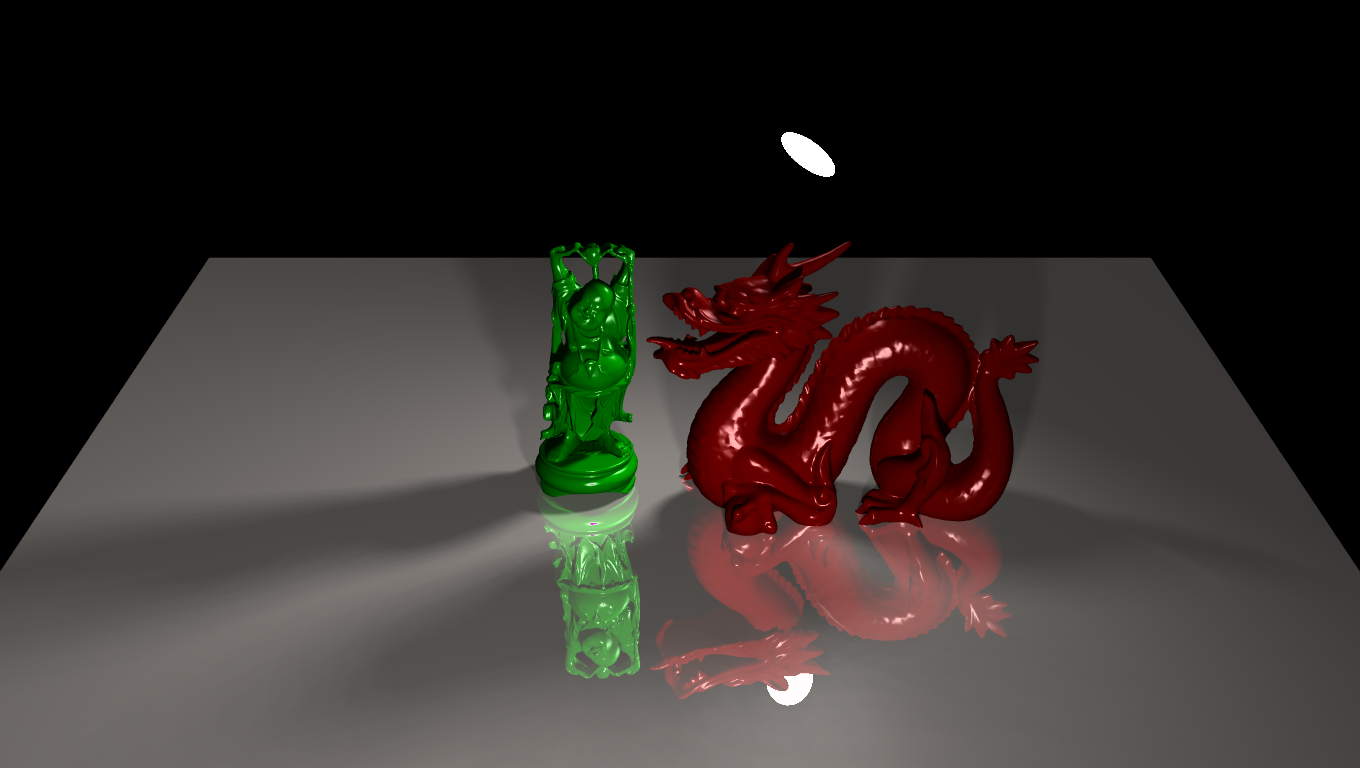
\includegraphics[width=1\textwidth]{./img/galerie/bhudda_dragon_glossy_plane_bright}
    \caption{Phong schattierter "`Stanford Buddha"' und "`Stanford Dragon"' auf spiegelndem Untergrund. Die Szene wird von zwei runden Flächenlichter beleuchtet.}
    \label{fig:bhudda_dragon_plane_glossy_bright}
\end{figure}



\begin{figure}[ht]
    \centering
    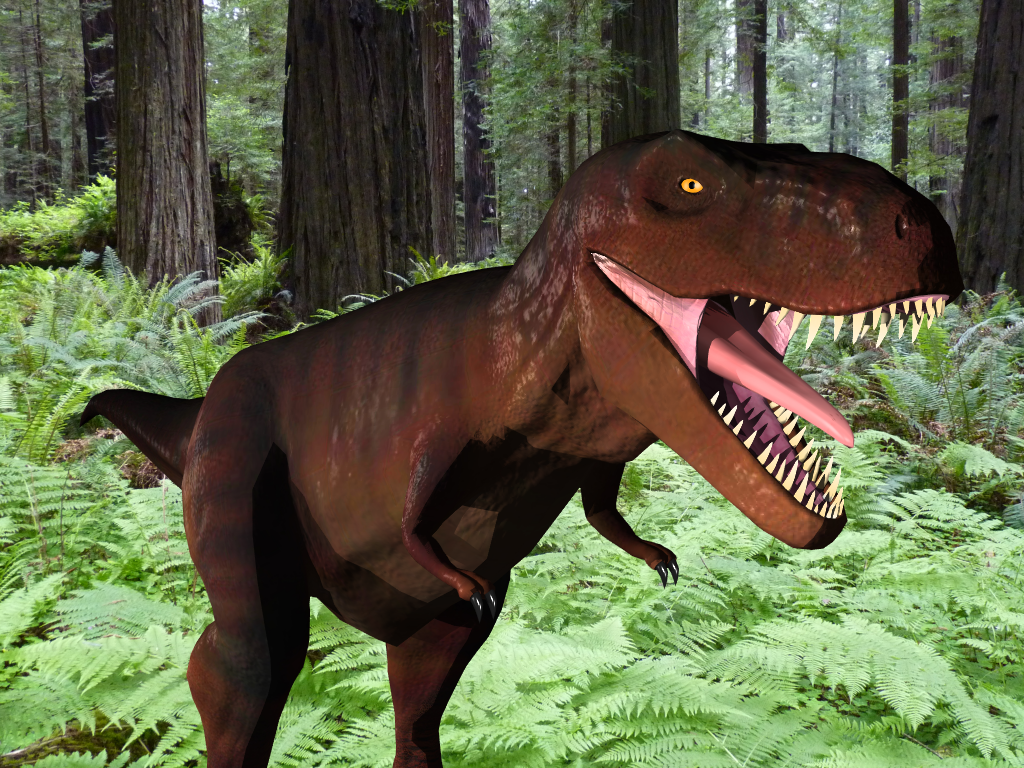
\includegraphics[width=1\textwidth]{./img/galerie/t-rex}
    \caption{Texturiertes Modell eines T-Rex, bestehend aus Bildtextur und "`Normal Map"'.}
    \label{fig:t-rex}
\end{figure}


\begin{figure}[ht]
    \centering
    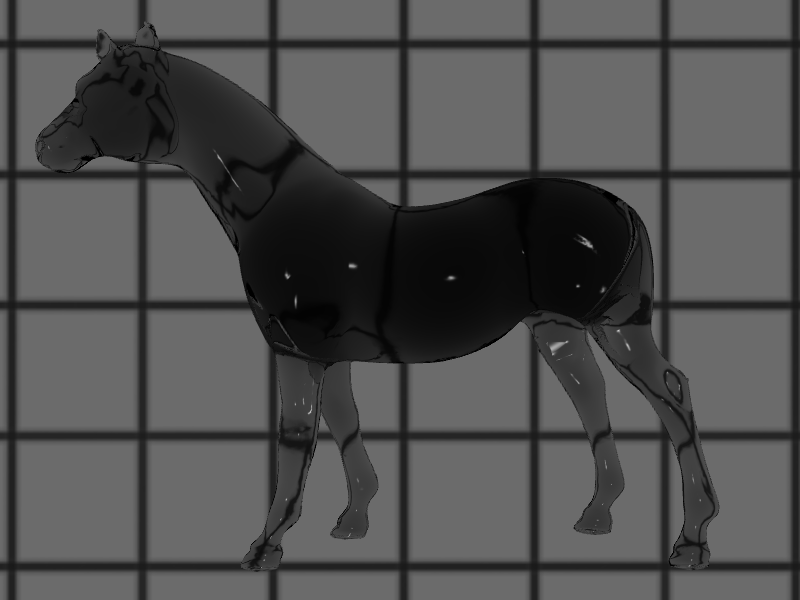
\includegraphics[width=1\textwidth]{./img/galerie/pferd_trans_dir.png}
    \caption{Pferdemodell gerendert mit dielektrischem Material unter Verwendung eines Brechungsindex von 1,3 und direktionalem Licht. Das Licht wird im Bauch des Pferdes stärker absorbiert als in den dünnen Beinen, wodurch diese dunkler wirkt.}
\end{figure}


\begin{figure}[ht]
    \centering
    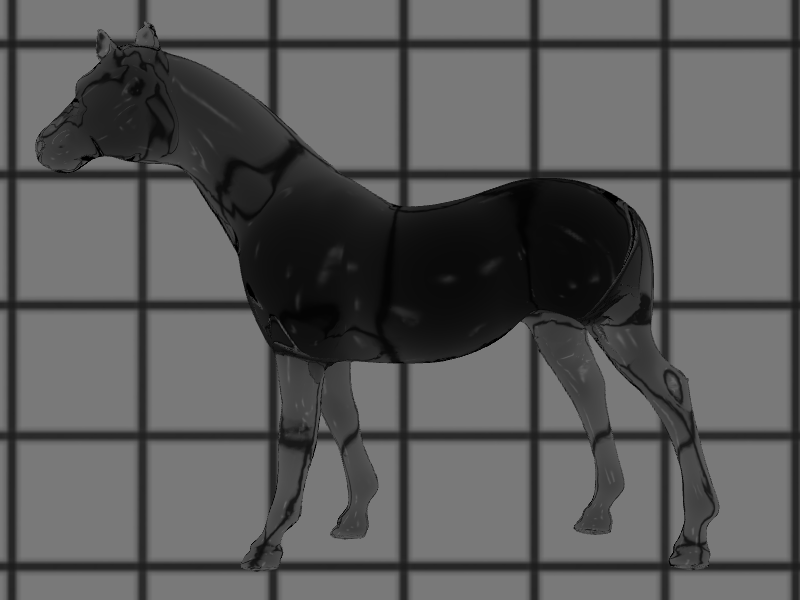
\includegraphics[width=1\textwidth]{./img/galerie/pferd_trans_flaeche.png}
    \caption{Pferdemodell gerendert mit dielektrischem Material unter Verwendung eines Brechungsindex von 1,3 und Flächenlicht. Das Licht wird im Bauch des Pferdes stärker absorbiert als in den dünnen Beinen, wodurch diese dunkler wirkt.}
\end{figure}

\begin{figure}[ht]
    \centering
    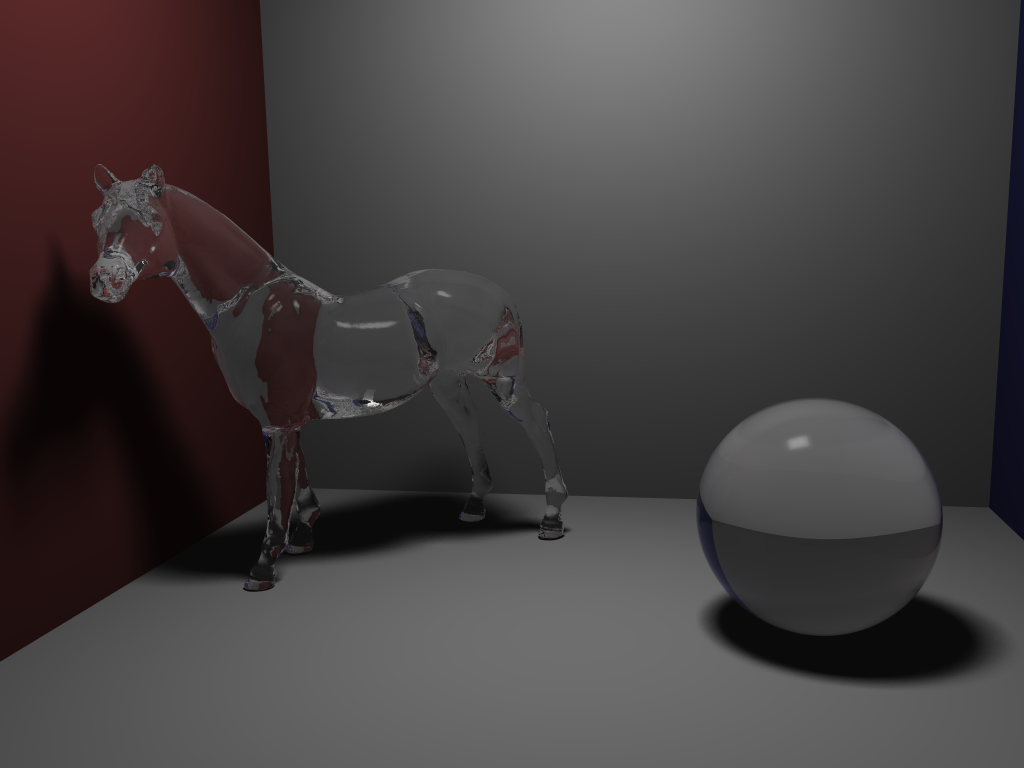
\includegraphics[width=1\textwidth]{./img/schattierung/dielectric_1_1,3.png}
    \caption{Pferdemodell und Kugel in "`Cornell box"'. Gerendert mit dielektrischem Material unter Verwendung eines Brechungsindex von 1,35 und Flächenlicht.}
\end{figure}

\begin{figure}[ht]
    \centering
    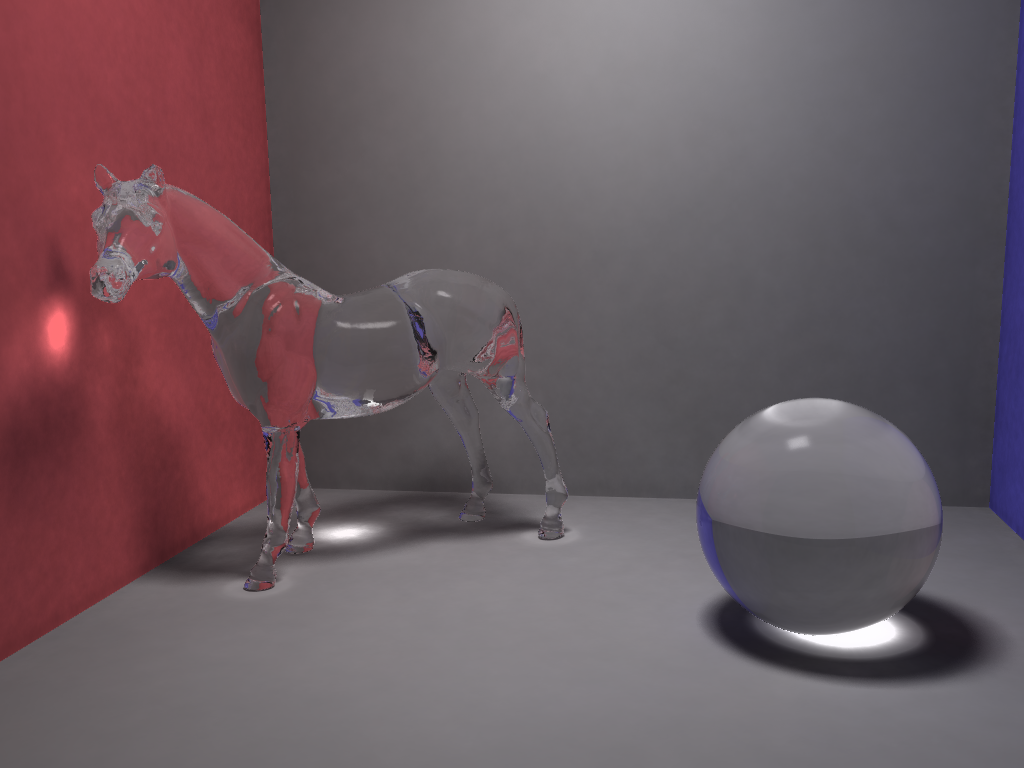
\includegraphics[width=1\textwidth]{./img/schattierung/dielectric_photon.png}
    \caption{Pferdemodell und Kugel in "`Cornell box"'. Gerendert mit dielektrischem Material unter Verwendung eines Brechungsindex von 1,35 und Flächenlicht. Verwendung von "`Photon Mapping"' mit 5 Millionen Photonen, zur Darstellung von Kaustiken und indirekter Beleuchtung. Zur Berechnung der Bestrahlungsstärke wurde eine konvexe Hülle verwendet, um dunkle Kanten und Ecken zu vermeiden.}
\end{figure}


\begin{figure}[ht]
    \centering
    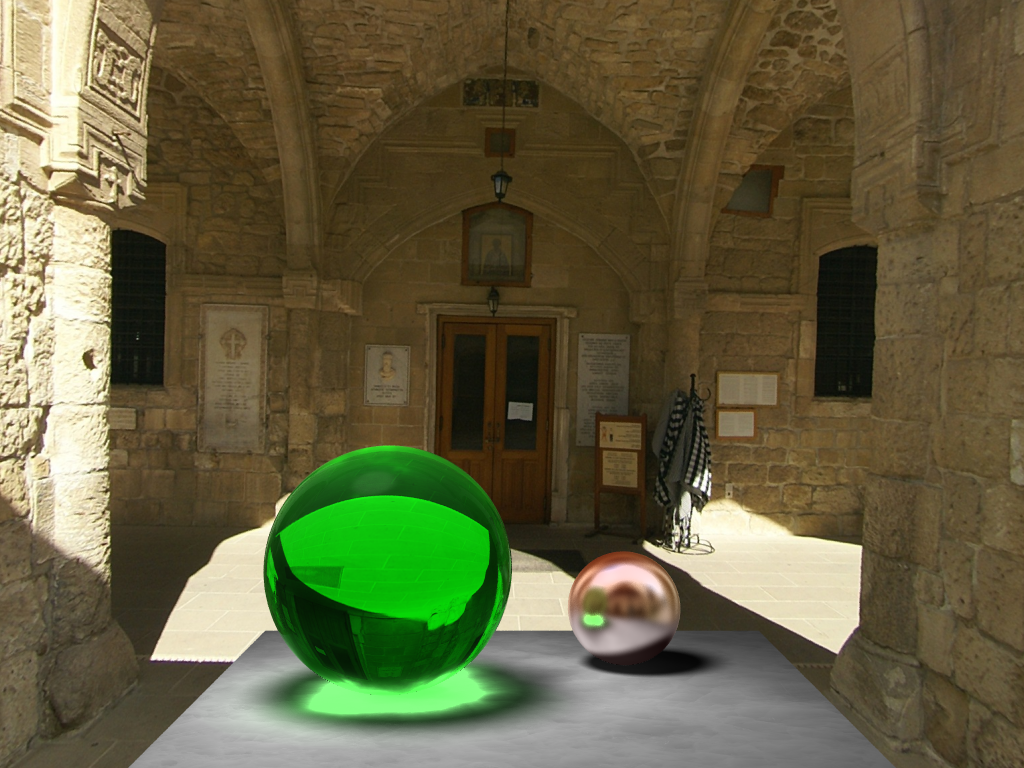
\includegraphics[width=1\textwidth]{./img/galerie/sphere_skybox_photon_clear}
    \caption{Transparente und matt spiegelnde Kugel in einer Skybox der Lazarus-Kirche. "`Photon Mapping"' erzeugt Kaustiken.}
    \label{fig:sphere_skybox_photon_clear}
\end{figure}



\begin{figure}[ht]
    \centering
    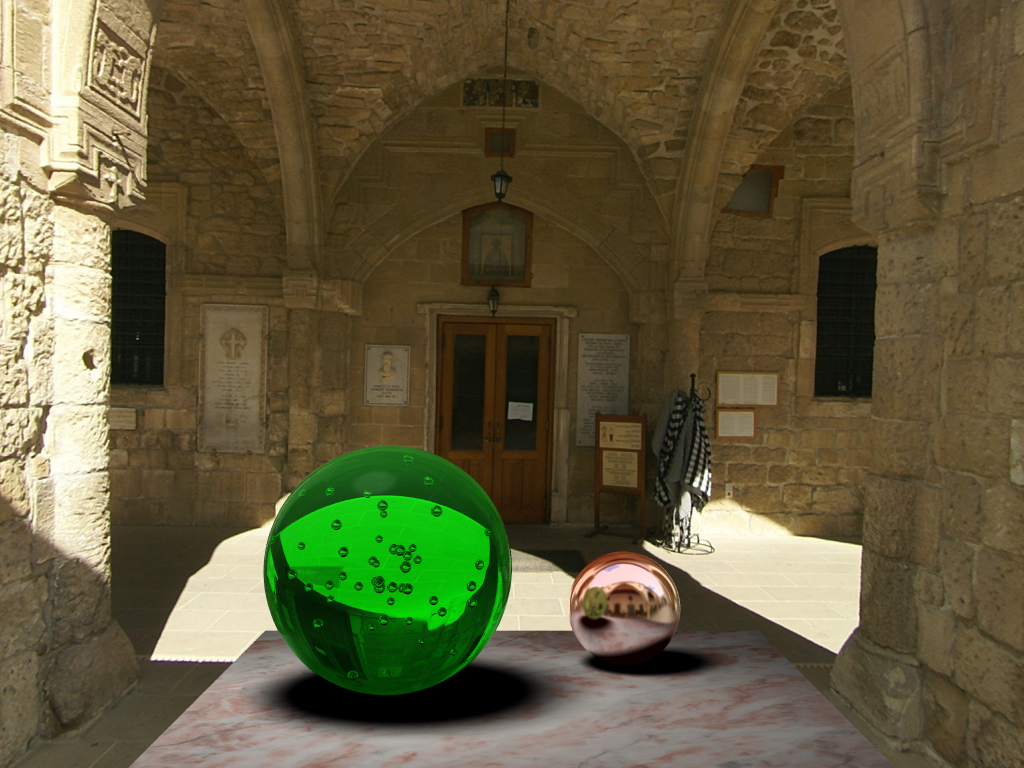
\includegraphics[width=1\textwidth]{./img/galerie/sphere_skybox_without_photon}
    \caption{Transparente Kugel mit eingeschlossen Luftblasen und spiegelnde Kugel in einer Skybox der Lazarus-Kirche.}
    \label{fig:sphere_skybox_photon_without_photon}
\end{figure}



\begin{figure}[ht]
    \centering
    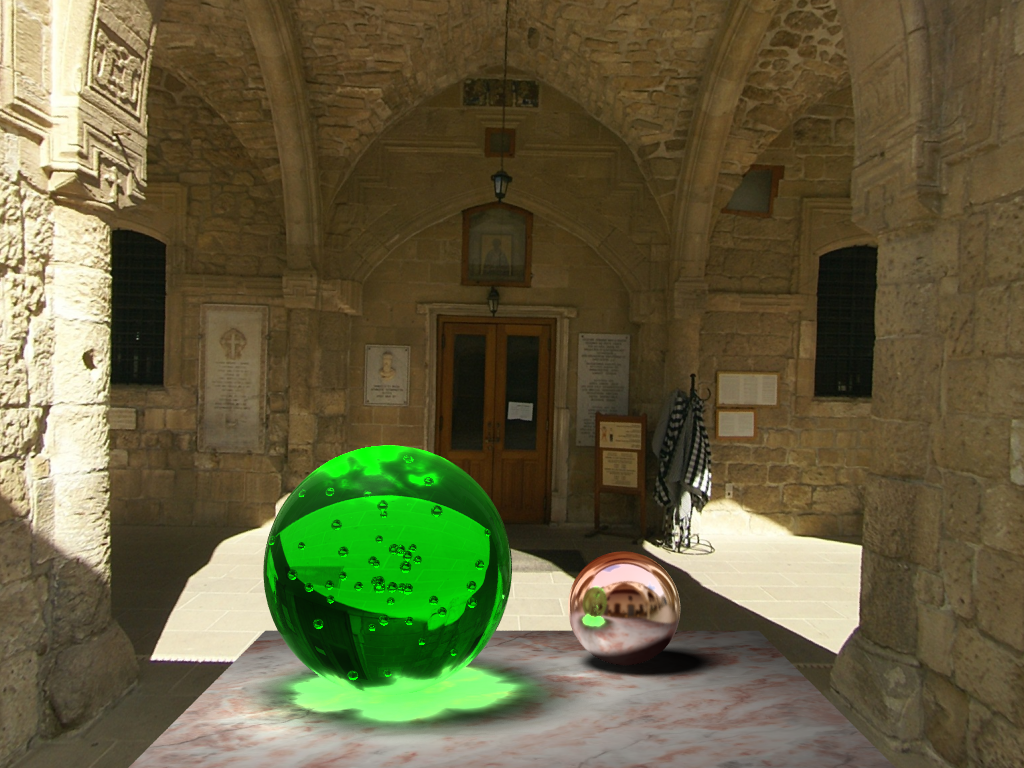
\includegraphics[width=1\textwidth]{./img/galerie/sphere_skybox_with_photon}
    \caption{Transparente Kugel mit eingeschlossen Luftblasen und spiegelnde Kugel in einer Skybox der Lazarus-Kirche. "`Photon Mapping"' sorgt für Kaustiken.}
    \label{fig:sphere_skybox_with_photon}
\end{figure}